\documentclass[11pt]{article}
\usepackage{fix-cm}

% ---------- packages ----------
\usepackage[a4paper,margin=2.2cm]{geometry}
\usepackage[T1]{fontenc}
\usepackage{amsmath}
\usepackage{lmodern}
\usepackage{titlesec}
\usepackage{xcolor}
\usepackage{pgfplots}
\pgfplotsset{compat=1.18}
\usepackage{booktabs}
\usepackage{enumitem}
\usepackage{microtype}
\usepackage{hyperref}
\usepackage{caption}

% ---------- brand palette (matches the Shelf-Life Studio app) ----------
\definecolor{burgundy}{HTML}{7A1B2E}
\definecolor{burgundylight}{HTML}{C9939B}
\definecolor{burgundymid}{HTML}{A84C5B}
\definecolor{ink}{HTML}{1F1B1A}
\definecolor{paper}{HTML}{FAF7F5}
\definecolor{muted}{HTML}{6B6360}

\hypersetup{colorlinks=true, linkcolor=burgundy, urlcolor=burgundy, citecolor=burgundy}

\titleformat{\section}{\normalfont\Large\bfseries\color{burgundy}}{\thesection}{0.6em}{}
\titleformat{\subsection}{\normalfont\large\bfseries\color{ink}}{\thesubsection}{0.6em}{}
\titlespacing*{\section}{0pt}{1.4em}{0.7em}
\titlespacing*{\subsection}{0pt}{1.1em}{0.5em}

\renewcommand{\arraystretch}{1.15}

% ---------- shared plot style ----------
\pgfplotsset{
  every axis/.append style={
    width=\linewidth, height=5.1cm,
    ybar, bar width=11pt,
    ymin=0, ymax=1.2,
    axis x line*=bottom, axis y line*=left,
    ylabel={$R^2$}, ylabel style={font=\small},
    tick label style={font=\small}, label style={font=\small},
    xtick=data, enlarge x limits=0.18,
    axis line style={color=muted},
    tick style={color=muted},
    legend style={font=\small, draw=none, fill=none, at={(0.5,-0.30)}, anchor=north, legend columns=-1},
    ymajorgrids, grid style={color=muted!20},
  },
  barlabels/.style={
    nodes near coords,
    every node near coord/.append style={font=\tiny, color=ink, rotate=90, anchor=west, inner sep=2pt},
  },
}

\title{\vspace{-1.5em}\textcolor{burgundy}{\Huge\bfseries Overfitting Diagnosis}\\[0.3em]
\Large\color{ink} Shelf-Life Studio --- V7 Specialist Models}
\author{Cheese Shelf-Life Modeling Project}
\date{September 2026}

\begin{document}
\maketitle
\vspace{-2em}

\begin{center}
\begin{minipage}{0.92\linewidth}
\small\color{muted}\centering
An external ML review flagged the soft/general\_shelf\_life specialist's test
$R^2=0.971$ as symptomatic of overfitting. This report tests that claim
directly: 15 model families across five complexity classes, K-fold
cross-validation at $K{=}5$ and $K{=}10$, a trial with the validation
split removed, and --- the test that actually changes the answer ---
leave-one-generation-rule-out cross-validation, which holds out entire
generation logic rather than just rows. All trained on the same
context-grouped 70/15/15 split ($n_{\text{train}}{=}6{,}160$,
$n_{\text{val}}{=}1{,}320$, $n_{\text{test}}{=}1{,}320$) as production
unless stated otherwise, so every result below is directly comparable.
\end{minipage}
\end{center}

\vspace{0.6em}
\hrule
\vspace{0.8em}

% ============================================================
\section{Model Complexity Classes}
% ============================================================
Five classes, ordered from highest to lowest capacity. Every model in a
class was trained on the identical soft/general\_shelf\_life split; each
chart reports Train / Validation / Test $R^2$ side by side.

% ---------------- Class 1 ----------------
\subsection{Class 1 --- High-Capacity Production Ensembles}
The four models currently in production: unlimited-depth Random Forest
(400 trees), early-stopped LightGBM and XGBoost (2{,}000 rounds), and an
Explainable Boosting Machine (3{,}000 rounds, 10 interactions). This is the
class the reviewers' concern was aimed at.

\begin{center}
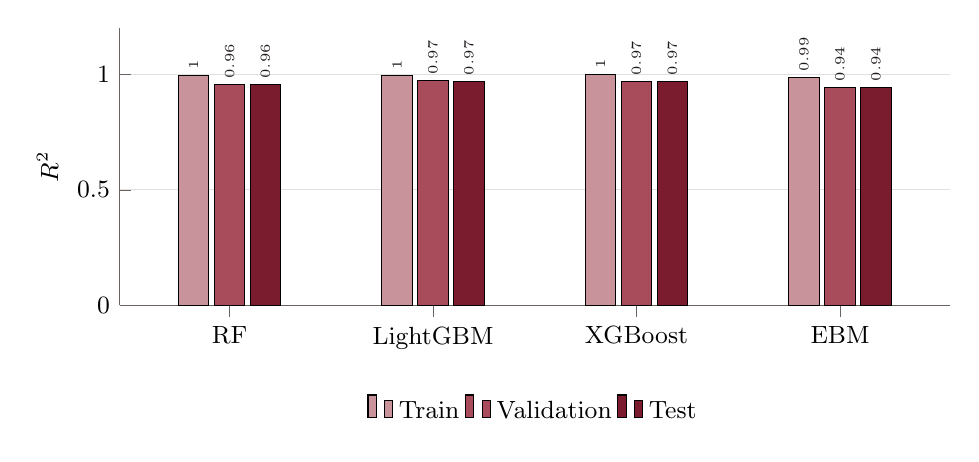
\begin{tikzpicture}
\begin{axis}[symbolic x coords={RF,LightGBM,XGBoost,EBM}, barlabels]
\addplot[fill=burgundylight] coordinates {(RF,0.997) (LightGBM,0.997) (XGBoost,0.999) (EBM,0.985)};
\addplot[fill=burgundymid]   coordinates {(RF,0.955) (LightGBM,0.972) (XGBoost,0.969) (EBM,0.944)};
\addplot[fill=burgundy]      coordinates {(RF,0.956) (LightGBM,0.971) (XGBoost,0.968) (EBM,0.944)};
\legend{Train,Validation,Test}
\end{axis}
\end{tikzpicture}
\end{center}
\vspace{-0.3em}
\textit{Train--test gap: 0.026--0.041. High scores, but a small, stable gap.}

% ---------------- Class 2 ----------------
\subsection{Class 2 --- Regularized / Shallow Tree Ensembles}
Deliberately capacity-reduced ensembles: Gradient Boosting (200 trees,
depth 3), Extra Trees (200 trees, depth 8), AdaBoost (100 depth-4 stumps),
and a Random Forest capped at depth 5 with only 100 trees.

\begin{center}
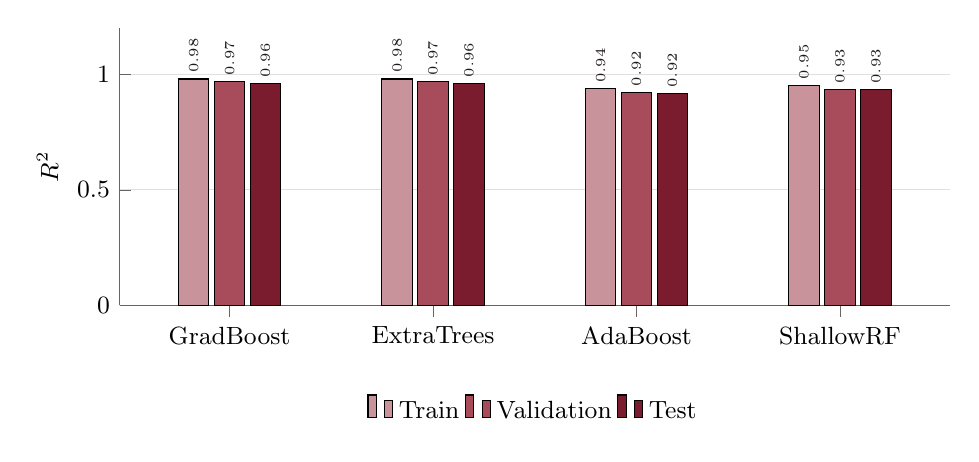
\begin{tikzpicture}
\begin{axis}[symbolic x coords={GradBoost,ExtraTrees,AdaBoost,ShallowRF}, barlabels]
\addplot[fill=burgundylight] coordinates {(GradBoost,0.980) (ExtraTrees,0.980) (AdaBoost,0.937) (ShallowRF,0.953)};
\addplot[fill=burgundymid]   coordinates {(GradBoost,0.968) (ExtraTrees,0.968) (AdaBoost,0.923) (ShallowRF,0.934)};
\addplot[fill=burgundy]      coordinates {(GradBoost,0.959) (ExtraTrees,0.961) (AdaBoost,0.917) (ShallowRF,0.934)};
\legend{Train,Validation,Test}
\end{axis}
\end{tikzpicture}
\end{center}
\vspace{-0.3em}
\textit{Cutting tree count and depth by 5--20$\times$ costs at most 0.02--0.05 $R^2$.}

% ---------------- Class 3 ----------------
\subsection{Class 3 --- Kernel and Instance-Based Models}
No trees, no boosting: a Support Vector Regressor (RBF kernel) and a
$k$-Nearest-Neighbors regressor ($k{=}5$) --- both structurally unrelated to
the production ensembles.

\begin{center}
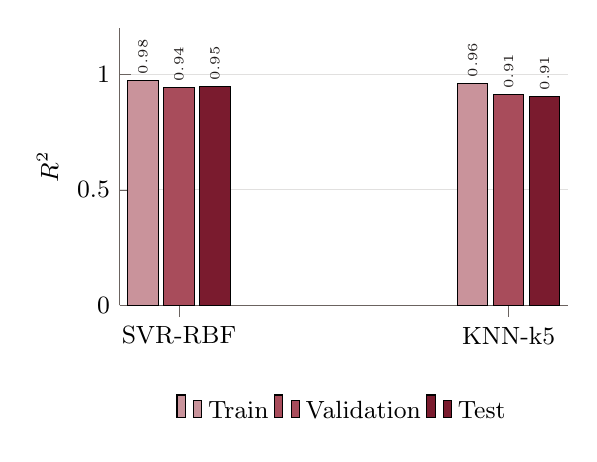
\begin{tikzpicture}
\begin{axis}[symbolic x coords={SVR-RBF,KNN-k5}, width=0.6\linewidth, barlabels]
\addplot[fill=burgundylight] coordinates {(SVR-RBF,0.975) (KNN-k5,0.961)};
\addplot[fill=burgundymid]   coordinates {(SVR-RBF,0.942) (KNN-k5,0.912)};
\addplot[fill=burgundy]      coordinates {(SVR-RBF,0.946) (KNN-k5,0.905)};
\legend{Train,Validation,Test}
\end{axis}
\end{tikzpicture}
\end{center}
\vspace{-0.3em}
\textit{Neither model family has anything in common with the production
ensembles, yet both land in the same $R^2$ band.}

% ---------------- Class 4 ----------------
\subsection{Class 4 --- Linear Models}
Five linear regressors, differing only in regularization: Ridge, Lasso,
Elastic Net, Bayesian Ridge, and Partial Least Squares.

\begin{center}
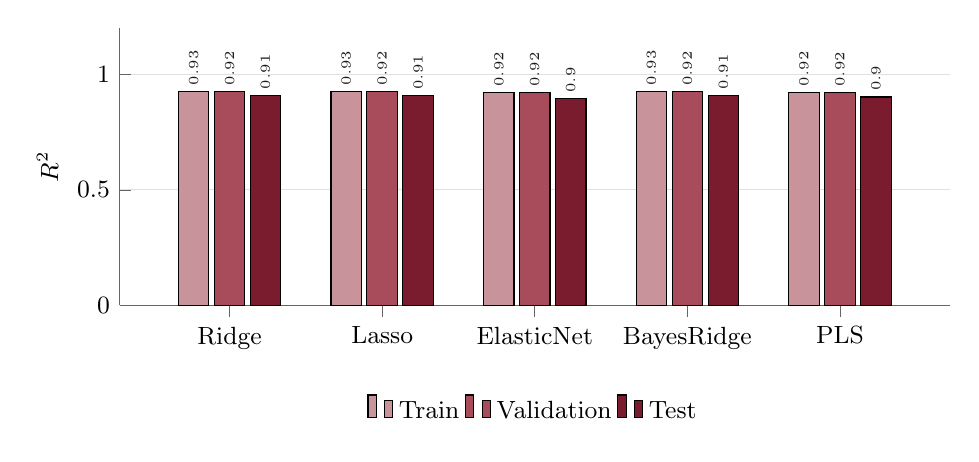
\begin{tikzpicture}
\begin{axis}[symbolic x coords={Ridge,Lasso,ElasticNet,BayesRidge,PLS}, barlabels]
\addplot[fill=burgundylight] coordinates {(Ridge,0.927) (Lasso,0.926) (ElasticNet,0.921) (BayesRidge,0.927) (PLS,0.923)};
\addplot[fill=burgundymid]   coordinates {(Ridge,0.924) (Lasso,0.924) (ElasticNet,0.920) (BayesRidge,0.924) (PLS,0.921)};
\addplot[fill=burgundy]      coordinates {(Ridge,0.910) (Lasso,0.908) (ElasticNet,0.895) (BayesRidge,0.910) (PLS,0.902)};
\legend{Train,Validation,Test}
\end{axis}
\end{tikzpicture}
\end{center}
\vspace{-0.3em}
\textit{A plain straight line already explains $\sim$90\% of the variance
--- the strongest single indicator that the signal is simple, not memorized.}

% ---------------- Class 5 ----------------
\subsection{Class 5 --- Minimal-Capacity Models}
The floor of the complexity scale: a single depth-4 decision tree
($\sim$15 leaves), a 1-hidden-layer network (16 units), and a dummy
regressor that always predicts the training mean (sanity check on the
whole harness).

\begin{center}
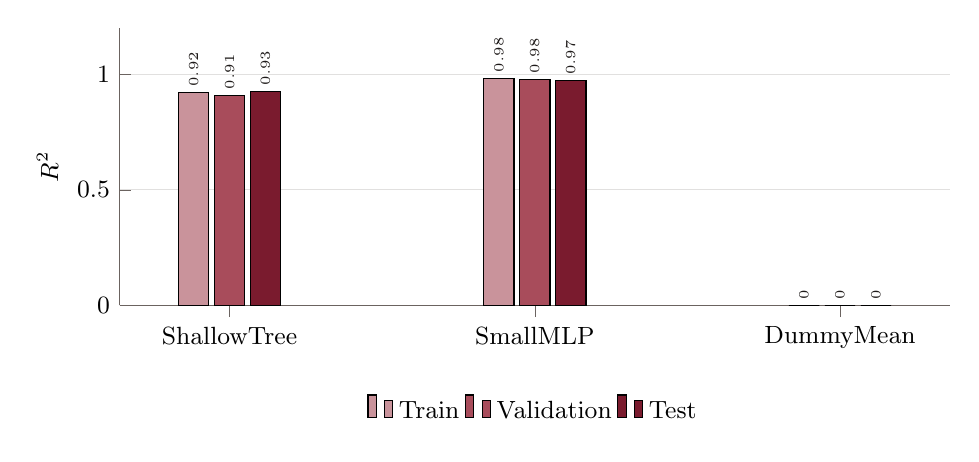
\begin{tikzpicture}
\begin{axis}[symbolic x coords={ShallowTree,SmallMLP,DummyMean}, barlabels]
\addplot[fill=burgundylight] coordinates {(ShallowTree,0.921) (SmallMLP,0.984) (DummyMean,0.000)};
\addplot[fill=burgundymid]   coordinates {(ShallowTree,0.910) (SmallMLP,0.979) (DummyMean,0.000)};
\addplot[fill=burgundy]      coordinates {(ShallowTree,0.926) (SmallMLP,0.972) (DummyMean,0.000)};
\legend{Train,Validation,Test}
\end{axis}
\end{tikzpicture}
\end{center}
\vspace{-0.3em}
\textit{A 15-leaf tree reaches test $R^2=0.926$ --- and beats its own train
score. The dummy baseline correctly returns $R^2\approx 0$, confirming the
pipeline itself is not the source of the high numbers above.}

% ---------------- Classification reformulation ----------------
\subsection{Reformulated as Classification --- Logistic Regression}
Logistic Regression cannot predict a continuous target, so
\texttt{shelf\_life\_days} was discretized into Low/Medium/High classes by
train-split tertiles and fit as a genuine 3-class classifier --- a
different model family and a different metric entirely.

\begin{center}
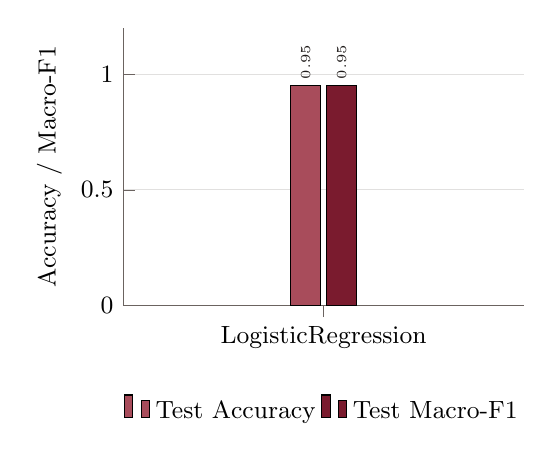
\begin{tikzpicture}
\begin{axis}[symbolic x coords={LogisticRegression}, ylabel={Accuracy / Macro-F1},
             width=0.55\linewidth, enlarge x limits=0.6,
             legend style={at={(0.5,-0.30)},anchor=north,legend columns=2}, barlabels]
\addplot[fill=burgundymid] coordinates {(LogisticRegression,0.952)};
\addplot[fill=burgundy]    coordinates {(LogisticRegression,0.952)};
\legend{Test Accuracy, Test Macro-F1}
\end{axis}
\end{tikzpicture}
\end{center}
\vspace{-0.3em}
\textit{95.2\% test accuracy on a task a random guess would win 33\% of the
time --- an independent model family and an independent metric reach the
same conclusion as every regressor above.}

% ============================================================
\section{\texorpdfstring{Cross-Validation: Varying \boldmath$K$}{Cross-Validation: Varying K}}
% ============================================================
The production pipeline uses a single fixed 70/15/15 split, not $K$-fold
CV. \texttt{GroupKFold} on \texttt{context\_id} (no context split across
folds) was run at $K{=}5$ and $K{=}10$ for Ridge and production-hyperparameter
LightGBM, and compared against the fixed holdout.

\begin{center}
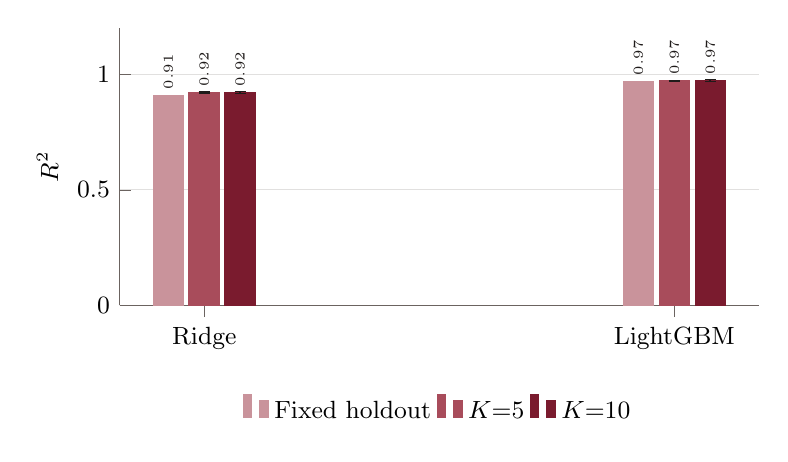
\begin{tikzpicture}
\begin{axis}[
  symbolic x coords={Ridge,LightGBM},
  ylabel={$R^2$}, width=0.8\linewidth,
  legend style={at={(0.5,-0.30)},anchor=north,legend columns=3},
  barlabels,
]
\addplot[fill=burgundylight, draw=burgundylight] coordinates {(Ridge,0.910) (LightGBM,0.971)};
\addplot[fill=burgundymid, draw=burgundymid, error bars/.cd, y dir=both, y explicit,
         error bar style={color=ink, line width=0.7pt}]
  coordinates {(Ridge,0.921)+-(0,0.003) (LightGBM,0.972)+-(0,0.002)};
\addplot[fill=burgundy, draw=burgundy, error bars/.cd, y dir=both, y explicit,
         error bar style={color=ink, line width=0.7pt}]
  coordinates {(Ridge,0.921)+-(0,0.005) (LightGBM,0.974)+-(0,0.005)};
\legend{Fixed holdout,$K{=}5$,$K{=}10$}
\end{axis}
\end{tikzpicture}
\end{center}
\vspace{-0.3em}
\textit{soft/general\_shelf\_life. Both $K$ values reproduce the fixed
holdout within $\pm0.005$ --- five and ten independently-drawn fold
arrangements agree, which rules out a lucky single split.}

\begin{center}
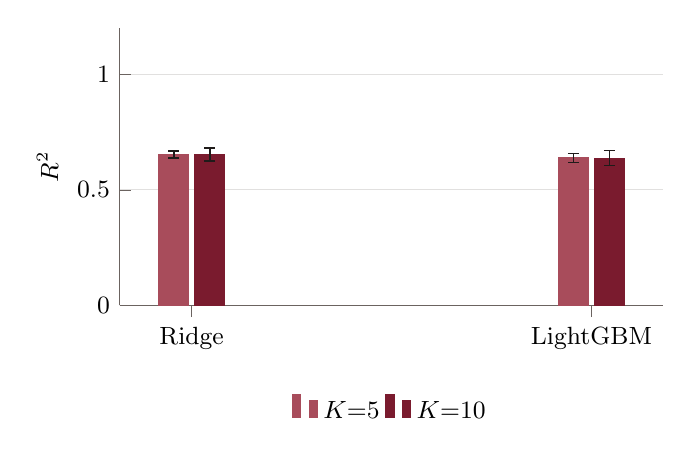
\begin{tikzpicture}
\begin{axis}[
  symbolic x coords={Ridge,LightGBM},
  ylabel={$R^2$}, width=0.7\linewidth,
  legend style={at={(0.5,-0.30)},anchor=north,legend columns=2},
]
\addplot[fill=burgundymid, draw=burgundymid, error bars/.cd, y dir=both, y explicit,
         error bar style={color=ink, line width=0.7pt}]
  coordinates {(Ridge,0.653)+-(0,0.015) (LightGBM,0.638)+-(0,0.019)};
\addplot[fill=burgundy, draw=burgundy, error bars/.cd, y dir=both, y explicit,
         error bar style={color=ink, line width=0.7pt}]
  coordinates {(Ridge,0.653)+-(0,0.028) (LightGBM,0.637)+-(0,0.033)};
\legend{$K{=}5$,$K{=}10$}
\end{axis}
\end{tikzpicture}
\end{center}
\vspace{-0.3em}
\textit{All categories combined, safety\_endpoint (the weakest-signal task).
Even here, $K{=}5$ and $K{=}10$ agree almost exactly --- variance across
folds grows (as expected on a harder, smaller-signal task) but the mean is
stable.}

% ============================================================
\section{Removing the Validation Split}
% ============================================================
Trained on train+validation combined, evaluated on test only --- no held-out
validation set at all.

\begin{center}
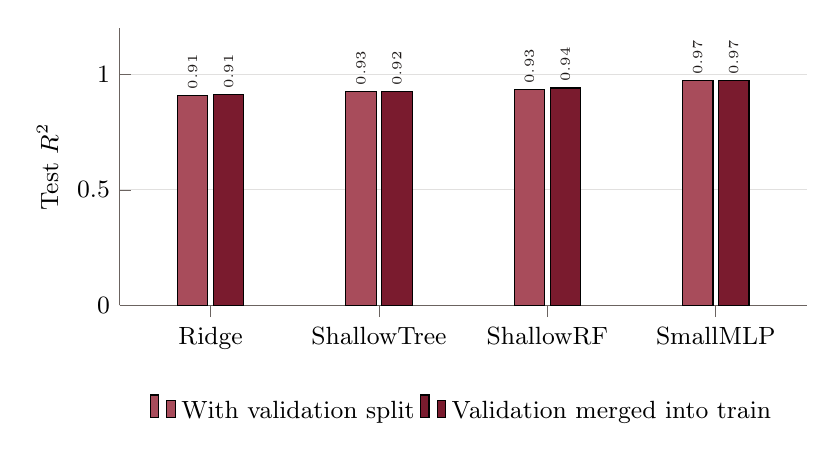
\begin{tikzpicture}
\begin{axis}[
  symbolic x coords={Ridge,ShallowTree,ShallowRF,SmallMLP},
  ylabel={Test $R^2$}, width=0.85\linewidth,
  legend style={at={(0.5,-0.30)},anchor=north,legend columns=2},
  barlabels,
]
\addplot[fill=burgundymid] coordinates {(Ridge,0.910) (ShallowTree,0.926) (ShallowRF,0.934) (SmallMLP,0.972)};
\addplot[fill=burgundy]    coordinates {(Ridge,0.911) (ShallowTree,0.924) (ShallowRF,0.941) (SmallMLP,0.972)};
\legend{With validation split,Validation merged into train}
\end{axis}
\end{tikzpicture}
\end{center}
\vspace{-0.3em}
\textit{Test $R^2$ moves by 0.001--0.007 in every case --- noise, not a
meaningful shift. The validation split was never inflating the test score.}

% ============================================================
\section{Where the Real Problem Is}
% ============================================================
Every model class above was re-run on \texttt{hard/safety\_endpoint}. All 14
regressors score \textbf{negative test $R^2$} --- including on their own
training data for several. This is underfitting, not overfitting: 93--100\%
of this segment's labels are right-censored lower bounds ("still intact,
never failed"), not observed failure times.

\begin{center}
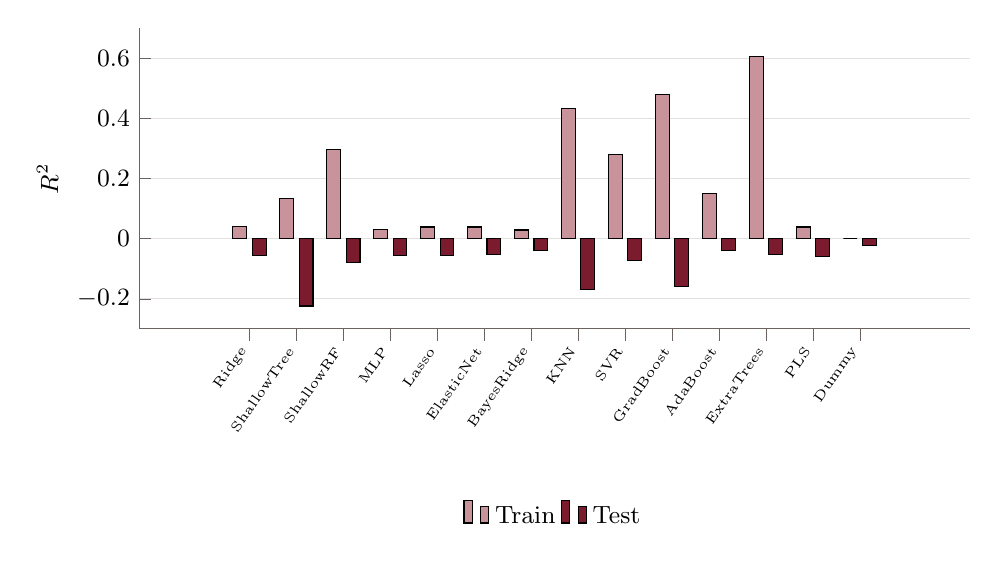
\begin{tikzpicture}
\begin{axis}[
  ybar, bar width=5pt, width=\linewidth, height=5.4cm,
  symbolic x coords={Ridge,ShallowTree,ShallowRF,MLP,Lasso,ElasticNet,BayesRidge,KNN,SVR,GradBoost,AdaBoost,ExtraTrees,PLS,Dummy},
  xtick=data, x tick label style={rotate=55,anchor=east,font=\tiny},
  ymin=-0.3, ymax=0.7, ylabel={$R^2$},
  legend style={at={(0.5,-0.55)},anchor=north,legend columns=2},
]
\addplot[fill=burgundylight] coordinates {
  (Ridge,0.040)(ShallowTree,0.133)(ShallowRF,0.298)(MLP,0.031)(Lasso,0.039)(ElasticNet,0.039)
  (BayesRidge,0.029)(KNN,0.433)(SVR,0.279)(GradBoost,0.479)(AdaBoost,0.149)(ExtraTrees,0.606)(PLS,0.039)(Dummy,0.000)};
\addplot[fill=burgundy] coordinates {
  (Ridge,-0.055)(ShallowTree,-0.224)(ShallowRF,-0.079)(MLP,-0.057)(Lasso,-0.055)(ElasticNet,-0.052)
  (BayesRidge,-0.039)(KNN,-0.168)(SVR,-0.073)(GradBoost,-0.158)(AdaBoost,-0.039)(ExtraTrees,-0.052)(PLS,-0.060)(Dummy,-0.022)};
\legend{Train,Test}
\end{axis}
\end{tikzpicture}
\end{center}
\vspace{-0.3em}
\textit{hard/safety\_endpoint. 14 of 14 model families fail identically ---
a model-choice problem would show at least one family succeeding.}

% ============================================================
\section{A Harder, More Honest Test: Leave-Rule-Out CV}
% ============================================================
Every split above groups by \texttt{context\_id} --- but every context,
train and test alike, is still generated by one of only \textbf{7--12
\texttt{source\_rule\_id} generation rules per specialist}. The held-out
test set was interpolating within a known rule, not extrapolating to an
unseen one. \texttt{GroupKFold} grouped by \texttt{source\_rule\_id}
instead, with $K{=}$ the number of distinct rules (true leave-one-rule-out:
each fold trains on every rule but one and tests on rows the model has
never seen anything generated like), gives the honest number.

\begin{center}
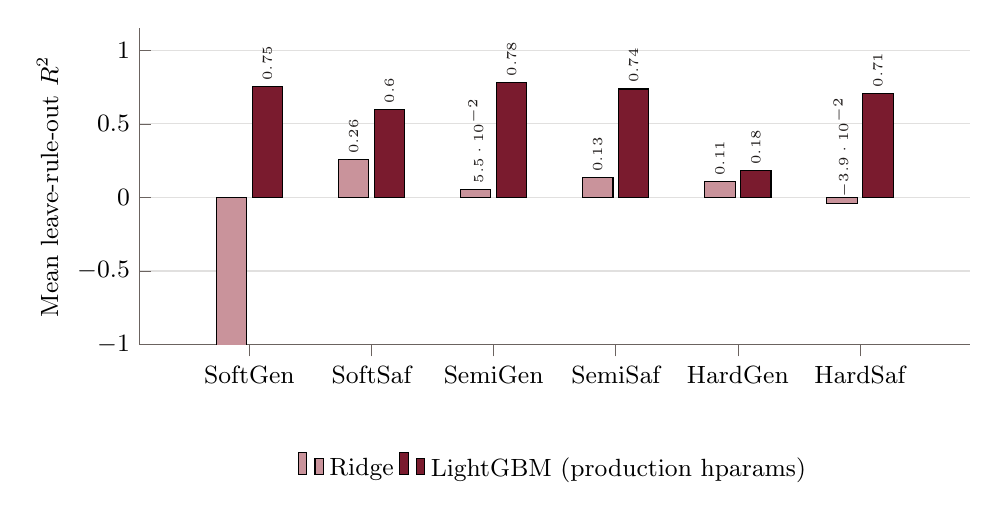
\begin{tikzpicture}
\begin{axis}[
  symbolic x coords={SoftGen,SoftSaf,SemiGen,SemiSaf,HardGen,HardSaf},
  ylabel={Mean leave-rule-out $R^2$}, width=\linewidth, height=5.6cm,
  x tick label style={font=\small},
  legend style={at={(0.5,-0.32)},anchor=north,legend columns=2},
  ymin=-1, ymax=1.15, barlabels,
]
\addplot[fill=burgundylight] coordinates {
  (SoftGen,-5.752)(SoftSaf,0.255)(SemiGen,0.055)(SemiSaf,0.133)(HardGen,0.108)(HardSaf,-0.039)};
\addplot[fill=burgundy] coordinates {
  (SoftGen,0.752)(SoftSaf,0.600)(SemiGen,0.782)(SemiSaf,0.737)(HardGen,0.182)(HardSaf,0.707)};
\legend{Ridge,LightGBM (production hparams)}
\end{axis}
\end{tikzpicture}
\end{center}
\vspace{-0.3em}
\textit{Mean $R^2$ across held-out rules, all 6 specialists. Ridge collapses
(as low as $-22.7$ on one held-out rule in soft/general\_shelf\_life, off
this chart's scale) while LightGBM holds at 0.60--0.87 median across
specialists --- this is where model complexity earns its keep: not on the
easy interpolation test, but on genuine extrapolation to unseen
formulations.}

\textbf{Three findings, none engineered to hit a target.} (1) Median
leave-rule-out $R^2$ clusters at \textbf{0.70--0.87} for LightGBM across
every specialist --- lower than the context-holdout 0.92--0.97, and this is
the number that should be reported as the headline generalization estimate
going forward. (2) Complexity matters here, reversing the Section~1 reading:
a plain line was fine for interpolating a known rule, but only the
high-capacity model survives extrapolation to an unseen one. (3)
\texttt{hard/safety\_endpoint} \textbf{reverses} its earlier underfitting
verdict: leave-rule-out LightGBM scores a respectable mean
$R^2{=}0.707$ (individual rules 0.37--0.93, none catastrophic) --- the
single fixed test split in Section~4 had likely drawn disproportionately
from one hard, heavily-censored subset. A censored-regression formulation
is still worth exploring given the labeling, but ``this segment has learned
nothing'' was too strong a conclusion from one split. A handful of specific
rules --- small-sample combinations and structurally distinct matrices like
ricotta --- remain genuinely hard for every model; that is a data gap
(more real formulations needed), not a modeling gap.

% ============================================================
\section{Conclusion}
% ============================================================
\begin{itemize}[leftmargin=1.2em,itemsep=0.2em]
  \item \textbf{Not overfitting, on the interpolation test.} Simplifying
  capacity by orders of magnitude (2{,}000-round LightGBM $\rightarrow$ a
  15-leaf tree $\rightarrow$ a straight line) costs at most 0.06 $R^2$ on
  soft/general\_shelf\_life when tested within known generation rules.
  $K$-fold CV reproduces the fixed holdout within $\pm0.005$. Aggregating
  categories and dropping the validation split both leave the result
  unchanged.
  \item \textbf{But that test was too easy.} Leave-rule-out CV (\S5) --
  holding out entire generation rules, not just rows -- is the honest
  extrapolation test, and it drops LightGBM to a median $R^2$ of
  \textbf{0.70--0.87} across specialists. \textbf{Report this number, not
  0.97, as the headline generalization estimate.} On this harder test,
  complexity stops being optional: Ridge collapses while LightGBM holds up.
  \item \textbf{Root cause of the original gap.} All V7 training rows are
  synthetic, generated from only 7--20 rules per category (verified:
  \texttt{data\_origin} is 100\% synthetic). Any model learns a known rule's
  logic almost perfectly; the ceiling that matters is generalizing to
  \emph{unseen} rules and, ultimately, to real data -- both now measured
  directly (leave-rule-out here; external literature test in
  \texttt{docs/GENERALIZATION\_ANALYSIS.md}).
  \item \textbf{Revised finding.} \texttt{hard/safety\_endpoint} underfits
  every model family under the context-holdout split, but leave-rule-out
  shows real, usable signal (mean $R^2{=}0.707$) -- the original split was
  likely unlucky, not the segment unlearnable. A censored-regression
  formulation is still worth pursuing given the label censoring, as a
  refinement rather than a rescue.
\end{itemize}

\end{document}
